En este apéndice documentaremos todas las clases, métodos y atributos que se han utilizado en el lenguaje JavaScript. Estas han sido utilizadas para gestionar desde un nivel más alto de abstracción los distintos componentes de WebGL explicados en la sección \ref{section:componentes-wgl}, modificar el DOM de los documentos HTML y darle valores a las variables \verb|attribute| y, de forma dinámica, también a las variables \verb|uniform| del fragment shader. Los ficheros que aquí documentamos pueden ser todos ellos encontrados en \url{https://github.com/JAntonioVR/Geometria-Fractal/tree/main/static/js}, donde además de encontrar las funciones aquí descritas con su código fuente, también encontraremos la misma cabecera descriptiva que incluimos en este apéndice.

Presentamos también en (TODO insert referencia) un diagrama UML con las relaciones que tienen estas clases entre sí.

\section{Componentes de WebGL comunes a 2D y 3D}

Comenzaremos documentando las clases y métodos comunes a la visualización de fractales 2D y 3D. Por ejemplo, la estructura de los shaders es la misma, aunque cambia drásticamente el código fuente de un caso a otro. También se utiliza un mismo buffer de vértices inicial para el vertex shader y ciertas inicializaciones de la escena son exactamente las mismas.

\subsection{Fichero `shader.js'}

Fichero con el código relativo a una abstracción de un shader. Hay dos posibles tipos de Shader (\verb|ShaderType|): Vertex y Fragment (clase \verb|Shader|), que juntos forman lo que llamamos `Programa Shader' (clase \verb|ShaderProgram|).

\subsubsection{ShaderType}

Enumerado inmutable, de forma que un elemento de la clase Shader sólo puede tener un tipo: \verb|ShaderType.vertexShader| o \verb|ShaderType.fragmentShader|.

\subsubsection{Class `Shader'}
Clase que abstrae un shader de WebGL, entendiendo shader como el programa relativo a un vertex shader o a un fragment shader. 

\paragraph*{Atributos}
\begin{itemize}
    \item \verb|program: WebGLShader|. Programa shader compilado.
    \item \verb|source: string|. Código fuente.
    \item \verb|type: ShaderType|. Tipo de shader. Vertex o fragment.
\end{itemize}

\paragraph*{Métodos}
\begin{itemize}
    \item \verb|constructor|: A partir del contexto de WebGL, del código fuente y del tipo de Shader, este método crea y compila el vertex/fragment shader.
    
    \textbf{Argumentos}:
    \begin{itemize}
        \item \verb|gl: WebGLContext|. Contexto de WebGL.
        \item \verb|source: string|. Código fuente del shader.
        \item \verb|type: ShaderType|. Tipo de Shader, vertex o fragment.
    \end{itemize}
    \textbf{Devuelve}: Un elemento de la clase Shader inicializado.

    \item \verb|getProgram|: Getter del atributo program, de tipo WebGLShader.
\end{itemize}

\subsubsection{Class `ShaderProgram'}
Clase que representa una abstracción de un programa shader, formado por el enlazado de un vertex shader y un fragment shader.

\paragraph*{Atributos}
\begin{itemize}
    \item \verb|vertexShader: Shader|. Objeto de la clase shader que corresponde a un vertex shader.
    \item \verb|fragmentShader: Shader|. Objeto de la clase shader que corresponde a un fragment shader.
    \item \verb|program: WebGLProgram|. Programa shader ya inicializado a partir de la conjunción de vertex y fragment shader.
\end{itemize}

\paragraph*{Métodos}
\begin{itemize}
    \item \verb|constructor|: Utiliza el contexto de WebGL y dos instancias de la clase Shader, uno de tipo vertex y otro de tipo fragment para inicializar el programa shader definitivo.
    
    \textbf{Parámetros}
    \begin{itemize}
        \item \verb|gl: WebGLContext|. Contexto de WebGL.
        \item \verb|vs: Shader|. Vertex Shader.
        \item \verb|fs: Shader|. Fragment Shader.
    \end{itemize}
    \textbf{Devuelve}: Un elemento de la clase ShaderProgram inicializado.
    \item \verb|getShaderProgram|:Getter del atributo program, de la clase WebGLProgram.
\end{itemize}

\subsection{Fichero `buffer.js'}

Fichero que contiene una abstraccion de un buffer de datos de WebGL.

\subsubsection{Class `Buffer'}

Clase que contiene un atributo del tipo WebGLBuffer y encapsula el comportamiento relativo a la inicialización de un buffer de WebGL. 

\paragraph*{Atributos}
\begin{itemize}
    \item \verb|buffer: WebGLBuffer|. Buffer de WebGL que contendrá la información requerida.
\end{itemize}

\paragraph*{Métodos}
\begin{itemize}
    \item \verb|constructor|: A partir del contexto de WebGL y de un array de JavaScript, construye y almacena en un atributo un elemento de la clase WebGLBuffer.
    \textbf{Parámetros}
    \begin{itemize}
        \item \verb|gl: WebGLContext|. Contexto de WebGL.
        \item \verb|array: Array|. Array de JavaScript a partir del cual se crea el buffer.
    \end{itemize}
    \textbf{Devuelve}: Un elemento de la clase Buffer inicializado.
    
    \item \verb|getBuffer|: Getter del atributo buffer, de la clase WebGLBuffer.
\end{itemize}

\subsection{Fichero `scene.js'}

Este fichero contiene los atributos y métodos de la clase 'Scene', una clase abstracta que representa una escena 2D o 3D.

\subsubsection{Class `Scene'}
Es una clase abstracta que contiene el código común de una escena 2D y una 3D. No podremos por tanto declarar una variable que sea de tipo \verb|Scene|, tan sólo podremos utilizar clases que hereden de esta.

\paragraph*{Atributos}
\begin{itemize}
    \item \verb|context: WebGLContext|. Contexto de WebGL.
    \item \verb|shaderProgram: ShaderProgram|. Programa Shader utilizado para graficar la escena en el canvas.
    \item \verb|bufferInfo: Object|. Objeto tipo diccionario que almacena información sobre los buffer de datos.
\end{itemize}
\paragraph*{Métodos}
\begin{itemize}
    \item \verb|constructor|: A partir del código fuente del vertex shader y del fragment shader inicializa el contexto de WebGL, el programa Shader y el buffer de posiciones de los vertices que toma como entrada el vertex shader.
    
    \textbf{Parámetros}
    \begin{itemize}
        \item \verb|vsSource: string|. Código fuente del vertex shader
        \item \verb|fsSource: string|. Código fuente del fragment shader.
    \end{itemize}
    
    \textbf{Devuelve}: Nada, realmente este constructor no se puede llamar por si solo, únicamente tiene el código comun a escenas 2D y 3D.
    
    \item \verb|initShaderProgram|: Crea y compila el vertex shader y el fragment shader. A partir de estos dos shaders, se crea el programa shader.
    
    \textbf{Parámetros}
    \begin{itemize}
        \item \verb|vsSource: string|. Código fuente del vertex shader
        \item \verb|fsSource: string|. Código fuente del fragment shader.
    \end{itemize}
    
    \textbf{Devuelve}: El programa shader ya inicializado, de la clase \verb|ShaderProgram|.

    \item \verb|initBuffers|: Inicializa los buffer necesarios, en nuestro caso tan solo se trata del buffer de posiciones de los vértices que recibe el vertex shader.
    
    \textbf{Argumentos}: No acepta.
    
    \textbf{Devuelve}: Un Objeto de JavaScript cuyos campos son:
    \begin{itemize}
        \item \verb|positionBuffer: WebGLBuffer|. Buffer de posiciones.
        \item \verb|numFloatsPV: number|. Número de valores en coma flotante por cada vértice.
        \item \verb|numVertexes: number|. Némero de vértices que se almacenan en el buffer.
    \end{itemize}

    \item \verb|drawScene|: Método abstracto que en las clases que hereden de Scene tomará el shader, los buffer y los parámetros de la escena para visualizarla en el canvas.
    
    \item  \verb|checkGLError|: Método que comprueba si hay algún error de OpenGL, en cuyo caso lanza una excepción.
    
    \textbf{Argumentos}: No acepta.
    
    \textbf{Devuelve}: Nada, tan solo lanza la excepcion cuando sea necesario.
\end{itemize}


\section{Visualización de fractales 2D}

Con la sección anterior hemos aclarado que utilizaremos el mismo buffer de posiciones, las mismas clases para el programa shader y mucho código común para las escenas. Las diferencias fundamentales entre el código JavaScript dedicado al uso de WebGL para visualizar fractales 2D y 3D se encuentra en los parámetros de la escena y en las maneras de gestionar los eventos. En esta sección describiremos todos estos aspectos en lo relativo a escenas 2D.

Recordamos que durante todo el capítulo \ref{chap:fractales-2D} estuvimos principalmente describiendo el código del fragment shader, pues es este el que se ejecuta en cada píxel, de forma que identificábamos cada píxel del canvas con un punto del plano complejo $\C$ y calculábamos si éste pertenecía al conjunto de Mandelbrot o al conjunto de Julia que decidiéramos. Para ayudarnos a visualizar distintas regiones del plano, distintos conjuntos de Julia fijando diferentes constantes $c\in\C$ o cambiar el exponente de la función $P_{c,m}=z^m+c$ utilizamos variables \verb|uniform| que insistíamos que se asignaba su valor utilizando JavaScript. La clase que gestiona esa asignación de valores y el cambio de forma dinámica de los mismos es \verb|Scene2D|, de ahí el valor de esta clase. En concreto, y aunque ahora explicaremos su significado en relación con los atributos de la clase, las distintas variables \verb|uniform| que hemos utilizado en el shader (fichero `shader-wgl-fragment.js') son:

\begin{lstlisting}
uniform vec2 u_zoomCenter;
uniform float u_zoomSize;
uniform int u_maxIterations;
uniform vec2 u_juliaSetConstant;
uniform int u_order;
uniform int u_fractal;
\end{lstlisting}

Recordando y teniendo estos detalles en mente, procedemos a documentar la clase \verb|Scene2D|.

\subsection{Fichero `scene2D.js'}

Código respectivo a la clase Scene2D, que representa una escena en la que podemos visualizar fractales en 2D.

\subsubsection{Class `Scene2D'}

Es una clase que hereda de Scene y que contiene el código relativo a la creacion, parámetros, visualizado y gestion de una escena 2D en la cual representaremos fractales 2D en un canvas de WebGL.

\paragraph*{Atributos}
Además de los heredados de \verb|Scene|, contamos con los siguientes atributos.
\begin{itemize}
    \item \verb|parameters: Object|. Objeto (diccionario) de JavaScript con varios campos, estos campos guardan una estrecha relación con las variables \verb|uniform| descritas anteriormente, ya que albergan los valores que posteriormente se enviarán a la variable homónima. Estos campos son:
    \begin{itemize}
        \item \verb|zoomCenter: Array|. Punto en WC que se encuentra en el centro del canvas $(x_0,y_0)$.
        \item \verb|zoomSize: number|. Valor que representa cuanto zoom hacemos en la escena $(\lambda)$.
        \item \verb|maxIterations: number|. Número máximo de iteraciones que se fijan en los algoritmos para graficar conjuntos de Julia y Mandelbrot.
        \item \verb|delta: number|. Incremento que se suma o resta a la hora de desplazarse por la escena.
        \item \verb|juliaSetConstant: Array|. Valor complejo $c$ en la ecuación $P_{c,m}(z)=z^m + c$.
        \item \verb|order: number|. Exponente $m$ en la ecuación $P_{c,m}(z) = z^m + c$.
        \item \verb|fractal: number|. Si este parámetro vale 0 se visualizará el conjunto de Mandelbrot. Si valiera 1 se graficaría el conjunto de Julia asociado al campo \verb|juliaSetConstant|.
    \end{itemize}
    \item \verb|programInfo: Object|. Objeto que almacena información genérica relativa al programa:
    \begin{itemize}
        \item \verb|program: WebGLProgram|. Programa Shader ya inicializado.
        \item \verb|attribLocations: Object|. Localización en memoria de las variables \verb|attribute|.
        \item \verb|uniformLocations: Object|. Localización en memoria de las variables \verb|uniform|.
    \end{itemize}
    \item \verb|initialParameters: Object|. Objeto tipo diccionario que es una copia exacta de \verb|parameters|, salvo que es inmutable, de forma que se permite restaurar los parámetros por defecto en caso de que se desee.
\end{itemize}
\paragraph*{Métodos}
\begin{itemize}
    \item \verb|constructor|: A partir del código fuente del vertex y el fragment shader, llama al constructor de la clase 'Scene', el cual crea el programa shader y el buffer de posiciones de los vértices que maneja el vertex shader. Además inicializa el atributo \verb|parameters|, con los parámetros iniciales que maneja la escena. Se crea y se le dan valores al atributo \verb|programInfo| y se almacenan en el atributo \verb|initialParameters| los parámetros iniciales de la escena.
    \textbf{Parámetros}
    \begin{itemize}
        \item \verb|vsSource: string|. Código fuente del vertex shader.
        \item \verb|fsSource: string|. Código fuente del fragment shader.
    \end{itemize}
    
    \textbf{Devuelve}: Un objeto de la clase Scene2D con todos sus atributos inicializados.
    
    \item \verb|drawScene|: A partir de los parámetros actuales que se encuentren en el atributo \verb|parameters|, las variables \verb|attribute| y \verb|uniform|, se envían estos valores a WebGL y se visualiza la escena.
    
    \textbf{Argumentos}: No acepta, toda la información que necesita está en los atributos de la clase.
    
    \textbf{Devuelve}: No devuelve nada, visualiza la escena en el canvas.
    \item \verb|zoomIn|: Se reduce el parámetro zoomSize para ampliar la escena. También se reduce \verb|delta| para que los desplazamientos sean menos bruscos.
    \item \verb|zoomOut|: Se aumenta el parámetro zoomSize para alejar la escena. También se aumenta \verb|delta| para que los desplazamientos sean más notables.
    \item \verb|moveLeft|: Se reduce la primera coordenada de \verb|zoomCenter| para desplazar la escena a la izquierda.
    \item \verb|moveRight|: Se aumenta la primera coordenada de \verb|zoomCenter| para desplazar la escena a la derecha.
    \item \verb|moveUp|: Se aumenta la segunda coordenada de \verb|zoomCenter| para desplazar la escena hacia arriba.
    \item \verb|moveDown|: Se reduce la segunda coordenada de \verb|zoomCenter| para desplazar la escena hacia abajo.
\end{itemize}

\pagebreak
\textbf{Getters}
\begin{itemize}
    \item \verb|getFractal|: Getter del parámetro \verb|fractal|, de tipo number.
    \item \verb|getJuliaConstantX|: Getter de la primera componente del parámetro \verb|juliaSetConstant|, de tipo number.
    \item \verb|getJuliaConstantY|: Getter de la segunda componente del parámetro \verb|juliaSetConstant|, de tipo number.
    \item \verb|getMaxIterations|: Getter del parámetro \verb|maxIterations|, de tipo number.
    \item \verb|getOrder|: Getter del parámetro \verb|order|, de tipo number.
\end{itemize}
\textbf{Setters}
\begin{itemize}
    \item \verb|setFractal|: Setter del parámetro \verb|fractal|.
    \item \verb|setInitialParameters|: Método que restablece los parámetros del objeto \verb|parameters| a los valores iniciales.
    \item \verb|setJuliaConstantX|: Setter de la primera componente del parámetro \verb|juliaSetConstant|.
    \item \verb|setJuliaConstantY|: Setter de la segunda componente del parámetro \verb|juliaSetConstant|.
    \item \verb|setMaxIterations|: Setter del parámetro \verb|maxIterations|.
    \item \verb|setOrder|: Setter del parámetro \verb|order|.
\end{itemize}

\subsection{Fichero `fractals-2D.js'}

Fichero javascript que gestiona los eventos y los indicadores HTML del documento \verb|2D-fractals.html|, entendiendo estos últimos como los pequeños elementos del documento en los cuales escribimos el valor actual de un parámetro (véase el documento \verb|2D-fractals| y cualquier etiqueta \verb|input| para una mejor comprensión). En este archivo se declara y utiliza continuamente una variable global de la clase \verb|Scene2D|, ya que es ésta la que lleva toda la interacción entre WebGL y los parámetros modificables. Este fichero, por su parte, sirve como intermediario entre el `front-end' HTML y la escena.

No existen como tal clases, tan sólo métodos que se utilizan como gestores de eventos y una función \verb|main|, la cual se ejecuta al cargar la página y contiene la inicialización de los indicadores HTML, la asignación de los 'event listeners' y la primera visualización.

Por su parte, las funciones gestoras de eventos modifican el HTML si es necesario, llaman al setter necesario para cambiar el parámetro con el nuevo valor y llaman a \verb|drawScene| para redibujar la escena con los nuevos parámetros. Incluimos debajo un ejemplo en el caso del deslizador que permite cambiar el parámetro \verb|maxIterations|:

\begin{lstlisting}
// CAMBIAR NUMERO MAXIMO DE ITERACIONES
function changeMaxIterations(event){
    document.querySelector("#valorNIteraciones").innerHTML 
        = event.target.value;
    theScene.setMaxIterations(event.target.value);
    theScene.drawScene();
}
\end{lstlisting}

\section{Ray-Tracing y fractales 3D}

En el caso de escenas tridimensionales, en la memoria se puede apreciar que la complejidad se dispara, aunque realmente el grueso de la dificultad se haya en el fragment shader. En lo relativo a JavaScript es todo más sencillo, con la salvedad de que el número de parámetros sí que es mucho mayor en estos casos, pero la filosofía es exactamente la misma. Tenemos una clase \verb|Scene3D| que gestiona el paso de parámetros dinámicamente a WebGL, los visualizados y los cambios en estos valores. A su vez también contamos con un fichero \verb|fractals-3D.js| cuya función es bien parecida a la de \verb|fractals-2D.js| pero con su contexto: la gestión de eventos y la correcta modificación de indicadores HTML.

Cuando visualizamos el espacio tridimensional usando técnicas como ray-tracing el fragment shader es mucho más complejo, aunque recordemos que en este momento lo único que nos interesa son las variables \verb|uniform| y su identificación con los parámetros de la escena. Veámos las variables que tenemos en el archivo \verb|shader-mandelbub-fragment.js|, el cual contiene el código fuente del fragment shader utilizado y además es realmente una extensión de \verb|shader-ray-tracer-fragment.js|.

\begin{lstlisting}
uniform vec3 u_lookfrom;
uniform vec3 u_lookat;

uniform vec4 u_ka;
uniform vec4 u_kd;
uniform vec4 u_ks;
uniform float u_sh;

uniform vec4 u_lightColor0;
uniform vec4 u_lightColor1;
uniform bvec3 u_shadows;

uniform float u_epsilon;

uniform int u_fractal;
uniform vec4 u_juliaSetConstant;
uniform bool u_antiliasing;
uniform int u_nSamples;
\end{lstlisting}

Como en la sección anterior, explicaremos el significado de cada una de ellas y su relación con los parámetros de la escena. Algunas de ellas, como \verb|u_fractal| o \verb|u_juliaSetConstant| tienen significados muy similares a los que tenían sus análogas en dos dimensiones, veámoslo.

\subsection{Fichero `scene3D.js'}

Contiene el código respectivo a la clase \verb|Scene3D|, que representa una escena en la que podemos visualizar fractales en 3D.

\subsubsection{Class `Scene3D'}

Es una clase que hereda de \verb|Scene| y que contiene el código relativo a la creación, parámetros, visualizado y gestión de una escena 3D en la cual representaremos fractales 3D en un canvas de WebGL. 

En esta clase se gestiona además una cámara orbital. Es decir, nos permite movernos alrededor de un punto fijo, que es el origen $(0,0,0)$, acercar y alejar nuestra posición. Para esto, se mantiene un parámetro que son las coordenadas esféricas del punto $lookfrom=(\rho,\phi,\theta)$, ya que con editar estos tres parámetros estaríamos moviendonos hacia adelante o atrás, derecha o izquierda y arriba o abajo en torno al punto $(0,0,0)$.

También se cuenta con parámetros para gestionar el realismo de la escena mediante el parámetro $\varepsilon$ que usamos en ray-marching; un material cuyas propiedades son totalmente editables; dos fuentes de luz situadas en las direcciones $(-0.5, 0.5, 0.0)$ (luz 0) y $(0.5, 0.5, 0.0)$ (luz 1) a las cuales se les puede cambiar el color y si deben o no arrojar sombras y la posibilidad de lanzar varios rayos por píxel. Aclaramos que todas estas mejoras dan unos resultados muy buenos pero también son computacionalmente muy costosas, por lo que puede ralentizarse mucho el rendimiento.

Dicho esto, presentamos los atributos que nos ayudarán a manejar toda esta funcionalidad.

\paragraph{Atributos}
Además de los heredados de \verb|Scene|, contamos con los siguientes atributos.
\begin{itemize}
    \item \verb|parameters: Object|. Objeto (diccionario) de JavaScript con varios campos, estos campos guardan una estrecha relación con las variables \verb|uniform| descritas anteriormente, ya que albergan los valores que posteriormente se enviarán a la variable homónima. Estos campos son:
    \begin{itemize}
        \item \verb|lookfrom: Array|. Punto en el cual se sitúa el espectador en coordenadas de mundo.
        \item \verb|lookfromSpheric: Array|. Coordenadas esféricas del punto \verb|lookfrom|.
        \item \verb|lookat: Array|. Punto hacia el que mira el espectador en coordenadas de mundo.
        \item \verb|ka: Array|. Tupla RGBA que representa la reflectividad ambiental del material parametrizable con el que se graficará el objeto central de la escena.
        \item \verb|kd: Array|. Tupla RGBA que representa la reflectividad difusa del material parametrizable con el que se graficará el objeto central de la escena.
        \item \verb|ks: Array|. Tupla RGBA que representa la reflectividad especular del material parametrizable con el que se graficará el objeto central de la escena.
        \item \verb|sh: number|. Exponente de brillo especular del material parametrizable.
        \item \verb|lightColor0: Array|. Tupla RGBA que será la intensidad de la luz derecha.
        \item \verb|lightColor1: Array|. Tupla RGBA que será la intensidad de la luz izquierda.
        \item \verb|shadows: Array|. Tripleta booleana tal que si \verb|shadows[i]| es true la fuente de luz i-esima arrojará sombras.
        \item \verb|fractal: number|. Si este parámetro vale 1 se visualizará el conjunto de Mandelbub. Si vale 2 se visualizará el conjunto de Julia asociado al campo \verb|juliaSetConstant|. Si vale 3 se visualizara el conjunto de Mandelbrot 3D.
        \item \verb|juliaSetConstant: Array|. Cuaternio $c$ en la ecuacion $P_c(q) = q^2 + c$.
        \item \verb|epsilon: number|. Distancia mínima $\varepsilon$ utilizada en ray-marching para decidir cuándo un punto esta en la frontera del fractal.
        \item \verb|antiliasing: boolean|. Si es true se aplicará antiliasing a la escena. En caso contrario se trazará un único rayo por píxel.
        \item \verb|nSamples: number|. Valor entero que en caso de que \verb|antiliasing| sea true se lanzarán $nSamples^2$ rayos por píxel.
        \item \verb|delta: number|. Incremento que se suma o se resta a la hora de desplazarse por la escena.
    \end{itemize}
    \item \verb|programInfo: Object|. Objeto que almacena información genérica relativa al programa:
    \begin{itemize}
        \item \verb|program: WebGLProgram|. Programa Shader ya inicializado.
        \item \verb|attribLocations: Object|. Localización en memoria de las variables \verb|attribute|.
        \item \verb|uniformLocations: Object|. Localización en memoria de las variables \verb|uniform|.
    \end{itemize}

    Hay que aclarar que este objeto no es el mismo que el de \verb|Scene2D|, pues aunque la estructura sea la misma el objeto \verb|Shader| y las variables \verb|uniform| (y por tanto sus localizaciones) no son las mismas.
    \item \verb|initialParameters: Object|. Objeto tipo diccionario que es una copia exacta de \verb|parameters|, salvo que es inmutable, de forma que se permite restaurar los parámetros por defecto en caso de que se desee.
\end{itemize}
\paragraph{Métodos}
\begin{itemize}
    \item \verb|constructor|: A partir del código fuente del vertex y el fragment shader, llama al constructor de la clase 'Scene', el cual crea el programa shader y el buffer de posiciones de los vértices que maneja el vertex shader. Además inicializa el atributo \verb|parameters|, con los parámetros iniciales que maneja la escena. Se crea y se le dan valores al atributo \verb|programInfo| y se almacenan en el atributo \verb|initialParameters| los parámetros iniciales de la escena.
    \textbf{Parámetros}
    \begin{itemize}
        \item \verb|vsSource: string|. Código fuente del vertex shader.
        \item \verb|fsSource: string|. Código fuente del fragment shader.
    \end{itemize}
    \textbf{Devuelve}: Un objeto de la clase Scene3D con todos sus atributos inicializados.

    \item \verb|drawScene|: A partir de los parámetros actuales que se encuentren en el atributo \verb|parameters|, las variables \verb|attribute| y \verb|uniform|, se envían estos valores a WebGL y se visualiza la escena.
    \textbf{Argumentos}: No acepta, toda la información que necesita está en los atributos de la clase.
    \textbf{Devuelve}: No devuelve nada, visualiza la escena en el canvas.

    \item \verb|zoomIn|: Se reduce el modulo del vector que une el origen con el punto \verb|lookfrom| para acercar la escena.
    \item \verb|zoomOut|: Se aumenta el modulo del vector que une el origen con el punto \verb|lookfrom| para alejar la escena.
    \item \verb|moveLeft|: Se modifica el angulo $\phi$ de las coordenadas esféricas del punto \verb|lookfrom| para desplazar la escena a la izquierda.
    \item \verb|moveRight|: Se modifica el angulo $\phi$ de las coordenadas esfericas del punto lookfrom para desplazar la escena a la derecha.
    \item \verb|moveX|: Dada una cantidad `\verb|desp|', desplaza la cámara a la derecha o a la izquierda \verb|desp| unidades.

    \textbf{Argumentos}:
    \begin{itemize}
        \item \verb|desp: number|. Número entero (positivo o negativo) que indica el desplazamiento.
    \end{itemize}
    \item \verb|moveUp|: Se modifica el angulo $\theta$ de las coordenadas esféricas del punto \verb|lookfrom| para desplazar la escena hacia arriba.
    \item \verb|moveDown|: Se modifica el angulo $\theta$ de las coordenadas esféricas del punto \verb|lookfrom| para desplazar la escena hacia abajo.
    \item \verb|moveY|: Dada una cantidad `\verb|desp|', desplaza la cámara hacia arriba o hacia abajo \verb|desp| unidades.

    \textbf{Argumentos}:
    \begin{itemize}
        \item \verb|desp: number|. Número entero (positivo o negativo) que indica el desplazamiento.
    \end{itemize}
    \item \verb|changeShadow|: Si la componente $i$-ésima del parámetro shadow esta a false la pone a true y viceversa. Es una forma de activar o desactivar las sombras arrojadas provocadas por una fuente de luz concreta.
    \textbf{Argumentos:}
    \begin{itemize}
        \item \verb|i: number|: Índice de la luz cuyas sombras queremos activar o desactivar.
    \end{itemize}
    \item \verb|changeAntiliasing|: Cambia el valor booleano del parámetro \verb|antiliasing|. Es una forma de decirle al programa si queremos que se aplique o no antiliasing a los píxeles.
    \item \verb|#rescaleAngles|: Cuando se modifican los ángulos de las coordenadas esféricas es posible que se salgan del rango $[0, 2\pi]$. Esta función ajusta esos valores para que siempre se sitúen en el intervalo correcto.
\end{itemize}
\textbf{Getters}
\begin{itemize}
    \item \verb|getAntiliasing|: Getter del parámetro \verb|antiliasing|, de tipo booleano.
    \item \verb|getEpsilon|: Getter del parámetro \verb|epsilon|, de tipo number.
    \item \verb|getFractal|: Getter del parámetro \verb|fractal|, de tipo number.
    \item \verb|getJuliaConstant|: Getter del parámetro \verb|juliaSetConstant|, de tipo Array (cuaternio).
    \item \verb|getKa|: Getter del parámetro \verb|ka|, de tipo array (terna RGBA).
    \item \verb|getKd|: Getter del parámetro \verb|kd|, de tipo array (terna RGBA).
    \item \verb|getKs|: Getter del parámetro \verb|ks|, de tipo array (terna RGBA).
    \item \verb|getLightColor|: Getter del parámetro 'lightColorX' donde X puede ser 0 o 1 según el valor del argumento.
    
    \textbf{Argumentos}:
    \begin{itemize}
        \item \verb|i: number|. Si vale 0 se devuelve el parámetro \verb|lightColor0|, en cualquier otro caso se devuelve \verb|lightColor1|.
    \end{itemize}
    \item \verb|getNSamples|: Getter del parámetro \verb|nSamples|, de tipo number.
    \item \verb|getPosition|: Getter del parámetro \verb|lookfrom|, la posición del observador.
    \item \verb|getSh|: Getter del parámetro \verb|sh|, tipo number.
\end{itemize}
\textbf{Setters}
\begin{itemize}
    \item \verb|setEpsilon|: Setter del parámetro \verb|epsilon|.
    \item \verb|setFractal|: Setter del parámetro \verb|fractal|.
    \item \verb|setInitialParameters|: Metodo que restablece los parámetros a los valores por defecto.
    \item \verb|setJuliaConstant|: Setter del parámetro \verb|juliaSetConstant|.
    \item \verb|setKa|: Setter del parámetro \verb|ka| (reflectividad ambiental).
    \item \verb|setKd|: Setter del parámetro \verb|kd| (reflectividad difusa).
    \item \verb|setKs|: Setter del parámetro \verb|ks| (reflectividad especular).
    \item \verb|setLightColor|: Setter del parámetro \verb|lightColorX|, donde X depende del valor del argumento \verb|i|.
    
    \textbf{Argumentos}:
    \begin{itemize}
        \item \verb|i: number|. Si vale 0, se modifica la terna RGB de la luz 0, en otro caso se modifica la terna de la luz 1.
    \end{itemize}
    \item \verb|setNSamples|: Setter del parámetro \verb|nSamples|.
    
    \item \verb|setSh|: Setter del parámetro \verb|sh| (exponente de brillo).
\end{itemize}

\subsection{Fichero `fractals-3D.js'}

Fichero javascript que gestiona los eventos y los indicadores HTML del documento \verb|3D-fractals.html|. La metodología utilizada en este fichero es la misma que la empleada en el caso 2-dimensional, solo que al haber más parámetros modificables, también hay más elementos HTML, y por tanto más eventos que gestionar y más indicadores que editar. Esta vez utilizamos una variable global de la clase \verb|Scene3D| para gestionar toda la interacción entre WebGL y los parámetros modificables.

Tampoco existen clases, únicamente funciones manejadoras de eventos y la función \verb|main| que se ejecuta al cargar la página y contiene la inicialización de los indicadores HTML, la asignación de los 'event listeners' y la primera visualización.

Para no alargar innecesariamente este apéndice y para que el propio lector observe la metodología por sí mismo, lo invitamos a visitar el fichero completo en \url{https://github.com/JAntonioVR/Geometria-Fractal/blob/main/static/js/fractals-3D.js}.

\section{Diagrama de clases UML}

En la imagen \ref{fig:UML} podemos ver un diagrama de clases del código recién explicado. Si se desea ver en mayor detalle en \href{https://github.com/JAntonioVR/Geometria-Fractal/blob/main/memoria/img/UML.png}{\textcolor{blue}{este enlace}} puede encontrar el archivo en formato `png'.

\begin{figure} [ht]
\centering
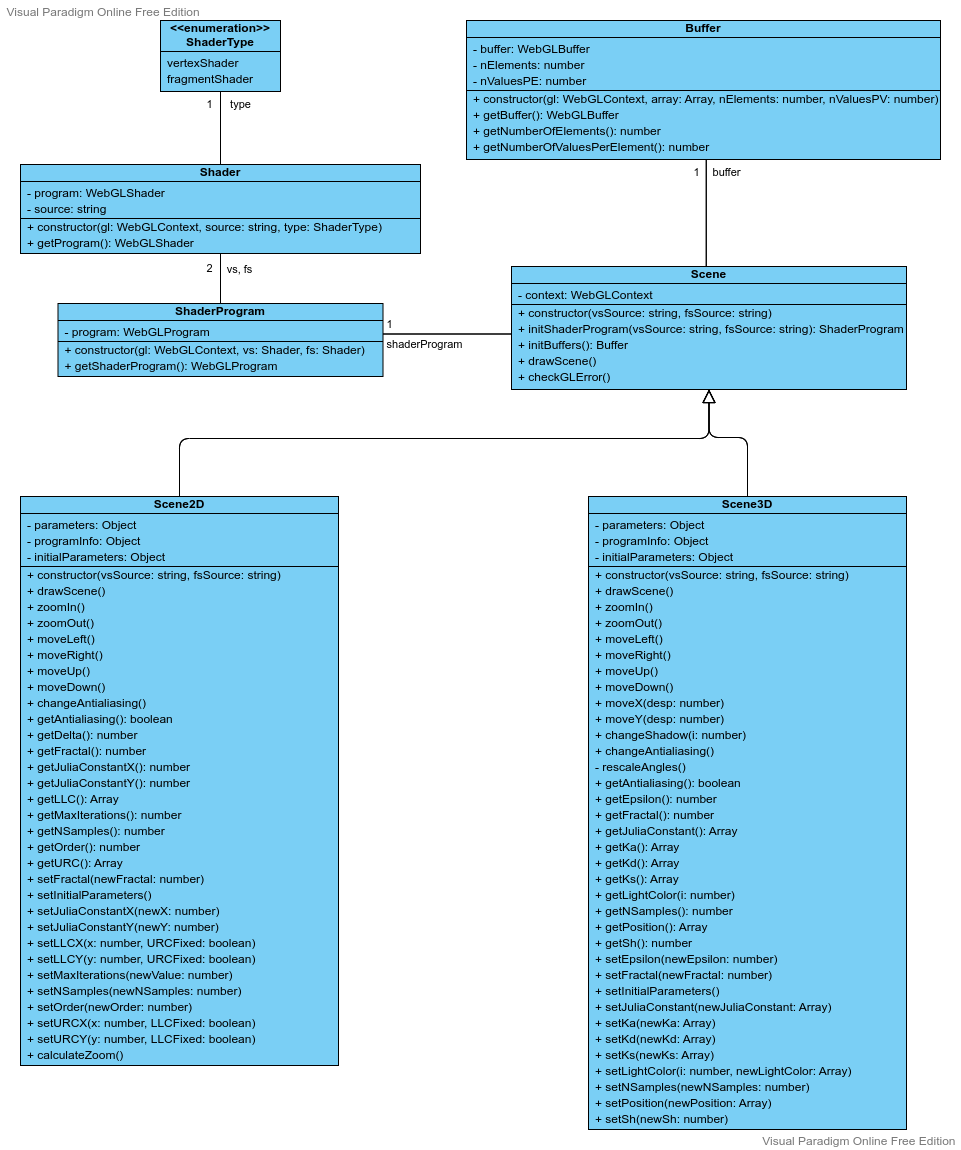
\includegraphics[scale = 0.45]{img/UML.png}
\caption{Diagrama de clases JavaScript utilizadas}
    \label{fig:UML}
\end{figure}